\documentclass[a4paper, 11pt]{article}
\usepackage[top=3cm, bottom=3cm, left = 2cm, right = 2cm]{geometry} 
\geometry{a4paper} 
\usepackage[utf8]{inputenc}
\usepackage{textcomp}
\usepackage{graphicx} 
\usepackage{amsmath,amssymb}  
\usepackage{bm}  
\usepackage[pdftex,bookmarks,colorlinks,breaklinks]{hyperref}  
\usepackage{listings}
\hypersetup{linkcolor=black,citecolor=black}
%\hypersetup{linkcolor=black,citecolor=black,filecolor=black,urlcolor=black} % black links, for printed output
\usepackage{memhfixc} 
\usepackage{pdfsync}  
\usepackage{fancyhdr}
\pagestyle{fancy}

\title{Creando un clon de Spotify con React Native}
\author{David Márquez Mínguez}

\begin{document}
\maketitle
\tableofcontents

\pagebreak
\section{Introducción}

\subsection{Contexto}

Este documento alberga todos los problemas que se me han planteado a la hora de construir un clon de Spotify utilizando
react-native. Además de ello, se incluirá en el mismo los pasos realizados y las decisiones tomadas para cada uno de los
desarrollos.

\subsection{Motivación}

La motivación principal para empezar el proyecto es aprender y mejorar mis habilidades como programador en el desarrollo
de aplicaciones.

\subsection{Objectivos y limitaciones}

Puesto que aún no soy un experto en este campo, seguro que surgirán errores en el análisis y desarrollo de las soluciones
propuestas. El objetivo de este documento no solo se  trata de aprender, sino de dejar evidenciado cada una de las
decisiones tomadas y mejorar al respecto.


\pagebreak
\section{Configuración del entorno de desarrollo}

Antes de comenzar el proyecto, el primer paso es la configuración del entorno. Para ello accedemos a la página oficial de
react-native y seguimos los pasos \cite{setup-development-environment}. En mi caso, puesto que ya he trabajado con alguna
aplicación móvil pequeña, no será necesaria mucha modificación.

Algo que si he tenido en cuenta y es importante comentar, es la eliminación del paquete \emph{@react-native-community/cli}.
La documentación aconseja su eliminación, ya que pueden surgir problemas inesperados, para ello ejecuto:

\begin{lstlisting}
    react-native-cli @react-native-community/cli
\end{lstlisting}

Antes e iniciar el proyecto, algo que es importante comentar es que React Native tiene una interfaz de línea de comandos
incorporada, esto significa que se puede generar un nuevo proyecto utilizando simplemente:

\begin{lstlisting}
    npx react-native@latest init src
\end{lstlisting}

Una vez iniciado el proyecto y con todos los paquetes necesarios instalados, precedemos a comprobar que la ejecución
funciona correctamente. Para ello nos creamos un dispositivo móvil virtual utilizando Android Studio. Una vez realizados
todos los pasos ejecutamos los comandos:

\begin{lstlisting}
    npm start
    npm run android
\end{lstlisting}

El primero inicia Metro, un paquete de JavaScript que se incluye con React Native. Este devuelve un solo archivo
JavaScript que incluye todo el código con sus dependencias. El segundo instala e inicia la aplicación en este caso en
Android.

\pagebreak
\section{Comienzo del desarrollo}

Una vez instalados todos los requerimientos previos y creado nuestro proyecto, comenzamos con el desarrollo.

\subsection{Construcción del sistema de navegación}

La primera funcionalidad a construir es el sistema de navegación entre pantallas. La aplicación va a tener un contenedor
inferior donde se mostrarán los iconos de \emph{'home', 'search' y your library'} y podremos ir cambiando de pantalla
según se vayan pulsando.

Para ello el primer paso es la instalacion del paquete \emph{@react-navigation/native} \cite{react-navigation}. Ejecutamos
el siguiente codigo y esperamos a que termine la instalación.

\begin{lstlisting}
    npm install @react-navigation/native
\end{lstlisting}

La propia construcción del sistema de navegación no tiene mucho misterio en sí, solo tenemos que meter las pantallas de
nuestra aplicación en el propio contenedor de navegación. Se muestra un código de ejemplo a continuación.

\begin{lstlisting}
    <NavigationContainer>
      <Tab.Navigator initialRouteName='Home'>
        <Tab.Screen
          name="Home"
          component={HomeScreen}/>
      </Tab.Navigator>
    </NavigationContainer>
\end{lstlisting}

En nuestro caso, puesto que tendremos tres pantallas principales, tendremos que crear otros dos componentes del tipo
Tab.Navigator, lo que supondrá la problemática de componentes dinámicos que se comentará más adelante.

Una vez definidos los componentes de navegación, queda darle estilo y agregar los iconos correspondientes a los mismos.
Para los estilos emplearé el mismo color de fondo que usa Spotify, así como el nombre de los botones. Para el tema de
los iconos usaré un paquete que no necesita previa instalación, \emph{'react-native-vector-icons}.

Para el uso de este paquete lo único que se debe hacer es modificar el archivo \emph{./android/app/build.gradle} y añadir
en la última línea \emph{apply from: ../../node\_modules/react-native-vector-icons/fonts.gradle} \cite{vector-icons-issue}.

\subsubsection{Creación de componentes dinamicos}

Cada uno de los iconos del sistema de navegación es un propio componente. ¿Hay que crear un componente distinto para
cada pantalla de la aplicación? ¿Qué ocurre entonces cuando queramos introducir iconos dependiendo del estado de enfoque?
La solución más sencilla a este problema es crear componentes dinámicos \cite{dynamic-components}.

Lo primero a definir es una constante que almacenara los componentes disponibles en función de los imports definidos. En 
este caso FoundationIcon, OcticonsIcon, EvilIcons y Ionicons son imports del paquete \emph{react-native-vector-icons}.

\begin{lstlisting}
    const iconComponents = {
        foundationIcon: FoundationIcon,
        octiconsIcon: OcticonsIcon,
        evilIcons: EvilIcons,
        ionicons: Ionicons
    }
\end{lstlisting}

Lo segundo es retornar el propio componente en cuestión. Para ello creo una función que dadas unas propiedades definidas 
por parámetro, cree ese componente a medida. El último paso será llamar al componente definido.

\begin{lstlisting}
    function MyIconComponent(props) {
        const MyComponent = iconComponents[props.component];
        return <MyComponent name={props.name} style={props.style} />;
    }
\end{lstlisting}

\subsection{Construcción de la primera pantalla}

a

\pagebreak

\section{Evaluation}

We did some experiments \ldots

\pagebreak

\section{Conclusions and Future Work}

From our experiments we can conclude that \ldots

\begin{figure}[tphb]
    \centering
    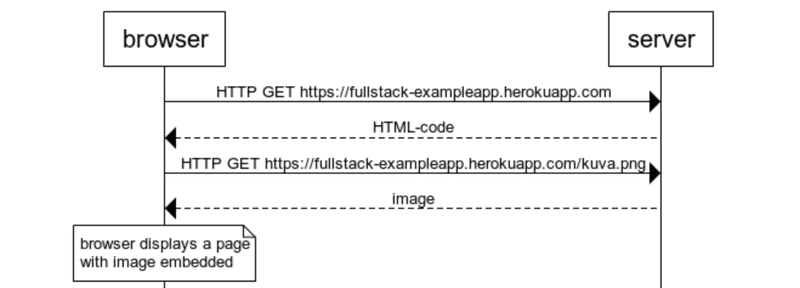
\includegraphics[width=7in]{img/testimg.png}
    \caption{testimg}
    \label{img:testimg}
\end{figure}

\pagebreak

\bibliographystyle{abbrv}
\bibliography{references}  % need to put bibtex references in references.bib 
\end{document}
